%%%%%%%%%%%%%%%%%%%%%%%%%%%%%%%%%%%%%%%%%%%%%%%%%%%%%
%				Overall architecture				%
%					-----------						%
% Author: Thibault Porteboeuf						%
%%%%%%%%%%%%%%%%%%%%%%%%%%%%%%%%%%%%%%%%%%%%%%%%%%%%%

\section{Overall Architecture}

The overall architecture is represented on figure \ref{archi}.
It comprises a LM32 core, some ROM and RAM memory that are represented using only one box on the figure, and video stream modules.

The video stream modules comprise VideoIn, which is responsible for handling the incoming video signals and store the frames to the RAM, VideoOut which is responsible for reading frames from mapped peripherals on the bus in order to generate video output signals, and finally the Coprocessor whose purpose is to process the video stream.

These different modules are connected together via a wishbone bus, represented in the center of the figure.

A module can be interfaced to the wishbone bus using two different kinds of interfaces: the slave interface or the master interface.

The master interface is intended for modules that need to initiate requests on the bus in order to get or post data to other modules.

The slave interface is intended for modules that need not to initiate requests on the bus, but only to handle incoming requests.

The interface's choice is thus made according to the module's role inside the system.

Some modules use only one interface. It is the case for the RAM and the LM32. The RAM only comprises a slave interface, since it just needs to handle read and write requests from the other modules.
On the other hand, the LM32 will never handle incoming requests from another module, but it will have to configure and control all these peripherals, therefore it comprises only a master interface.

The other modules, that is to say the video stream modules, comprise a master interface as well as a slave interface.
This is due to their particular role inside the system. They have a master module because they need to be able to retrieve and send video streams over the bus on their own, which allows the LM32 to perform other computations during this time.
They also have a slave interface, for they are the LM32's slaves. The LM32 really is the system's master, and has to configure all the other devices.
This slave interface the video stream modules have allows the LM32 to access and configure them via the bus, using \emph{configuration registers}.
These configuration registers and their implementation will be described later in this document.

As we explained, the LM32 initiates the requests that will configure all the peripherals. However, one could also notice the interrupt lines connected from the video stream modules to the LM32. The video processing modules will use these lines in order to notify the LM32 when a operation was completed successfully, and let it know that the video processing module now requires new instructions.

This process will be described later in details.

\begin{figure}[h]
	\center
	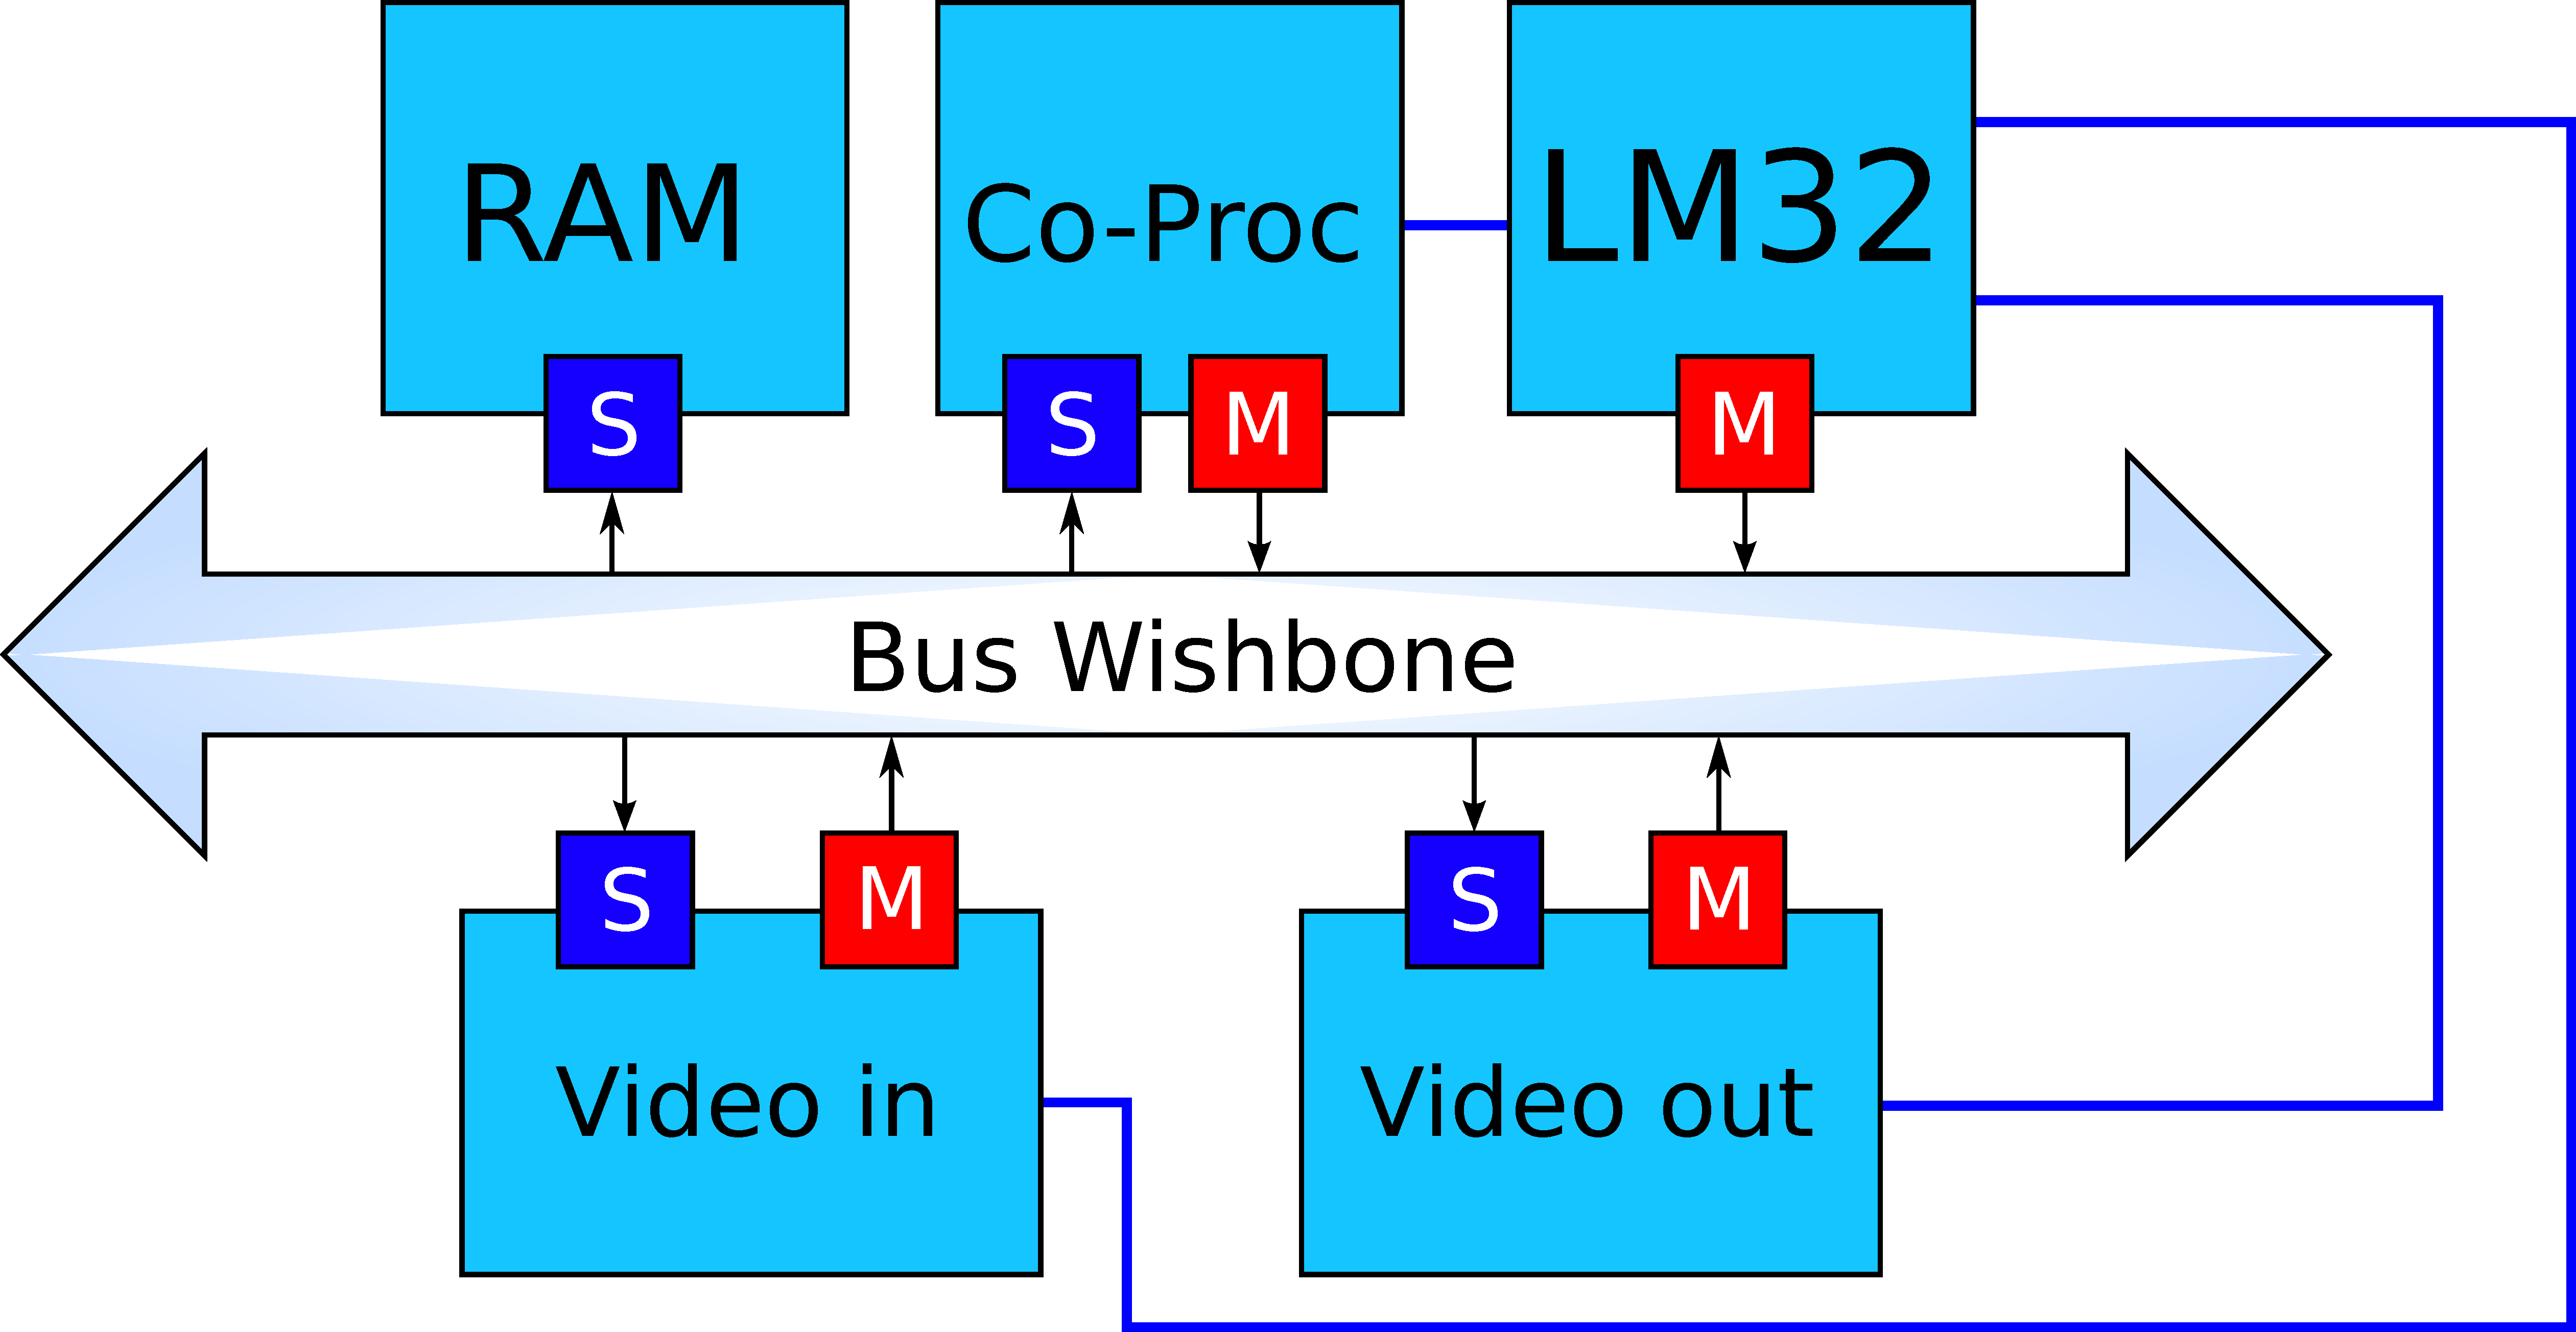
\includegraphics[width=11cm]{figs/overall_arch.pdf}

	\caption{Overall Architecture}
	\label{archi}
\end{figure}
